\documentclass[12pt, oneside]{article}
\usepackage[letterpaper, margin=1in, headsep=0.5in]{geometry}
\usepackage[english]{babel}
\usepackage[utf8]{inputenc}
\usepackage{amsmath}
\usepackage{amsfonts}
\usepackage{amssymb}
\usepackage{tikz}
\usetikzlibrary{quotes, angles}

\usepackage{fancyhdr}
\pagestyle{fancy}
\fancyhf{}
\rhead{\thepage \\}
\lhead{BECA / Dr. Huson / Mathematics\\* Template geometric figures}

\renewcommand{\headrulewidth}{0pt}

\begin{document}
\subsection*{Graphs}
tikz grid command

%Graph / grid
\begin{center}
  
\begin{tikzpicture}[scale=0.4] %[xscale=1,yscale=1]
  \draw[step=0.25in,gray,very thin] (0,0) grid (12.7,12.7);
  \end{tikzpicture}
\end{center} %Regents style, no axes

Axes
\begin{center} %4 quadrant regents grid
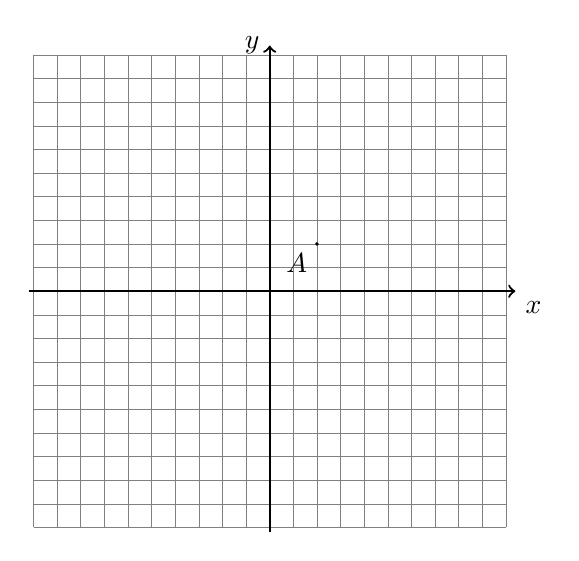
\begin{tikzpicture}[scale=.3]%[scale=0.635]
  \draw [help lines] (-10,-10) grid (10,10);
  \draw [thick, ->] (-10.2,0) -- (10.4,0) node [below right] {$x$};
  \draw [thick, ->] (0,-10.2)--(0,10.4) node [left] {$y$};
  \draw[fill] (2,2) circle  [radius=0.05]
       node[below left] (4, 2) {$A$};
\end{tikzpicture}
\end{center}

\begin{figure} %[!htbp] First quadrant with axes
  \caption{$x$ and $y$ axes for grid}
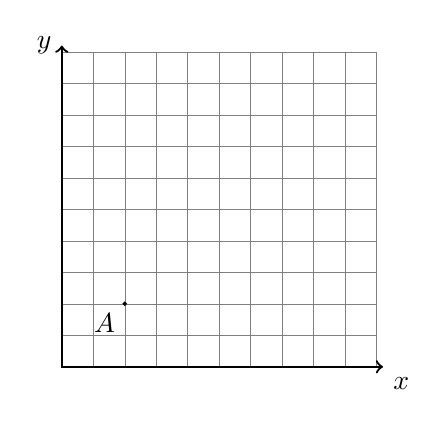
\begin{tikzpicture}[scale=0.4]
  \draw [help lines] (0,0) grid (10,10);
  \draw [thick, <->] (0,10.2) node [left] {$y$}
       -- (0,0) -- (10.2,0) node [below right] {$x$};
  \draw[fill] (2,2) circle  [radius=0.05]
       node[below left] (2, 2) {$A$};
\end{tikzpicture}
\end{figure}

\subsection*{Drawing lines and shapes}
tikz draw command, node labeling function\\
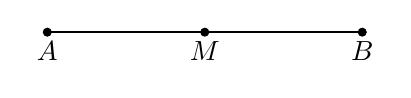
\begin{tikzpicture}
  \draw [-, thick] (1,0)--(5,0);
  \draw [fill] (1,0) circle [radius=0.05] node[below]{$A$};
  \draw [fill] (5,0) circle [radius=0.05] node[below]{$B$};
  \draw [fill] (3,0) circle [radius=0.05] node[below]{$M$};
\end{tikzpicture}

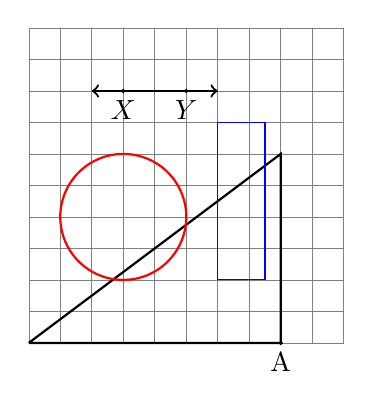
\begin{tikzpicture}[scale=0.4]
  \draw [help lines] (0,0) grid (10,10);
  %Triangle
  \draw [thick](0,0)--(8,0)--(8,6)--(0,0);
  \draw [fill] (8,0) circle [radius=0.05];
  \node [below] at (8,0) {A}; %above, right, left
  %line through points
  \draw [<->, thick] (2,8)--(6,8); % also thin, ultra thick, help lines, dashed, dotted, red
  \draw [fill] (3,8) circle [radius=0.05] node[below]{$X$};
  \draw [fill] (5,8) circle [radius=0.05] node[below]{$Y$};
  %shapes
  \draw [blue] (6,2) rectangle (7.5,7);
  \draw [red, thick] (3,4) circle [radius=2];
\end{tikzpicture}

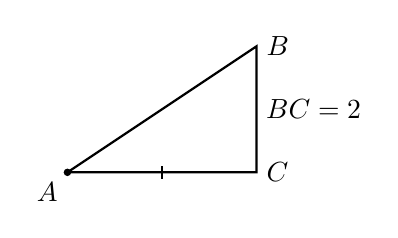
\begin{tikzpicture}[scale=0.8]
  \draw[fill] (2,2) circle  [radius=0.05]
       node[below left] (2, 2) {$A$};
  \draw [thick] (2,2)--(5,2) node[right] {$C$} --(5,4) node[right] {$B$} --(2,2);
  \draw [thick] (3.5,2.1)--(3.5,1.9); %tick mark
  \node [right] at (5,3) {$BC=2$};
\end{tikzpicture}

Given $\triangle ABC$ with $\overline{AC} \cong \overline{BC}$. $AC=x+7$ and $BC=2x+1$. Find $AC$.\\[0.5cm]
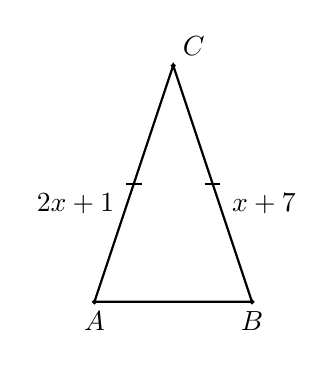
\begin{tikzpicture}[scale=0.5]
  \draw [thick](0,0)--(4,0)--(2,6)--(0,0);
  \draw [fill] (0,0) circle [radius=0.05] node[below]{$A$};
  \draw [fill] (4,0) circle [radius=0.05] node[below]{$B$};
  \draw [fill] (2,6) circle [radius=0.05] node[above right]{$C$};
  \draw [thick] (0.8,3)--(1.2,3); %tick mark
  \draw [thick] (2.8,3)--(3.2,3); %tick mark
  \node [right] at (3.25,2.5){$x+7$};
  \node [left] at (0.75,2.5){$2x+1$};
\end{tikzpicture}

\begin{center}
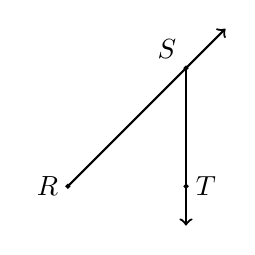
\begin{tikzpicture}[scale=0.5]
  \draw [->, thick] (0,0)--(4,4);
  \draw [->, thick] (3,3)--(3,-1);
  \draw [fill] (0,0) circle [radius=0.05] node[left]{$R$};
  \draw [fill] (3,3) circle [radius=0.05] node[above left]{$S$};
  \draw [fill] (3,0) circle [radius=0.05] node[right]{$T$};
\end{tikzpicture}
\end{center}

Given the rectangle $ABCD$ with $\overline{AB} \cong \overline{CD}$ and $\overline{BC} \cong \overline{DA}$. $AB=x+7$ and $\displaystyle CD=\frac{4x+2}{2}$. Find $AB$.\\[0.5cm]
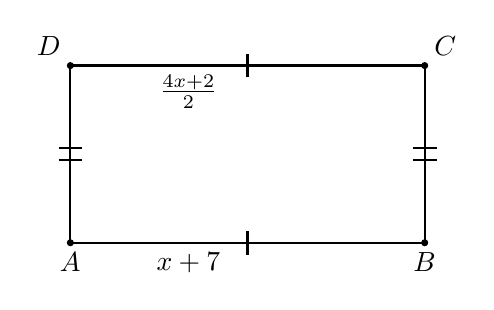
\begin{tikzpicture}[scale=0.75]
  \draw [thick](0,0)--(6,0)--(6,3)--(0,3)--(0,0);
  \draw [fill] (0,0) circle [radius=0.05] node[below]{$A$};
  \draw [fill] (6,0) circle [radius=0.05] node[below]{$B$};
  \draw [fill] (6,3) circle [radius=0.05] node[above right]{$C$};
  \draw [fill] (0,3) circle [radius=0.05] node[above left]{$D$};
  \draw [thick] (3,-0.2)--(3,0.2); %tick mark
  \draw [thick] (3,2.8)--(3,3.2); %tick mark
  \draw [thick] (-0.2,1.4)--(0.2,1.4); %tick mark
  \draw [thick] (-0.2,1.6)--(0.2,1.6); %tick mark
  \draw [thick] (5.8,1.4)--(6.2,1.4); %tick mark
  \draw [thick] (5.8,1.6)--(6.2,1.6); %tick mark
  \node [below] at (2,0){$x+7$};
  \node [below] at (2,3){$\frac{4x+2}{2}$};
\end{tikzpicture}

\subsection*{Plane geometry}
  Identify two lines in the given plane.\\
  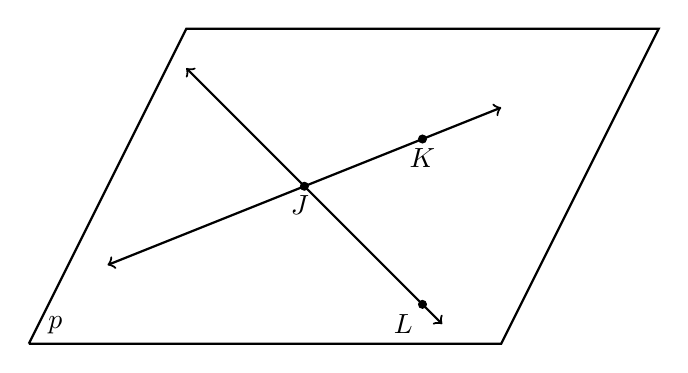
\begin{tikzpicture}
    \draw [thick](0,0) node[above right]{$\ p$} --(6,0)--(8,4)--(2,4)--(0,0);
    \draw [<->, thick] (1,1)--(6,3);
    \draw [fill] (3.5,2) circle [radius=0.05] node[below]{$J \ $};
    \draw [fill] (5,2.6) circle [radius=0.05] node[below]{$K$};
    \draw [<->, thick] (2,3.5)--(5.25,.25);
    \draw [fill] (5,0.5) circle [radius=0.05] node[below left]{$L$};
  \end{tikzpicture} \vspace{2cm}

\subsection*{Marking angles}
\tikz \draw (2,0) coordinate (A) -- (0,0) coordinate (B)
         -- (1,1) coordinate (C)
  pic ["$K$", draw, ->] {angle=A--B--C};

  \begin{tikzpicture}
    \draw
      (3,-1) coordinate (a) node[right] {a}
      -- (0,0) coordinate (b) node[left] {b}
      -- (2,2) coordinate (c) node[above right] {c}
      pic["$\alpha$", draw=orange, <->, angle eccentricity=1.2, angle radius=1cm]
      {angle=a--b--c};
  \end{tikzpicture}


\end{document}
